\documentclass{article}
\usepackage[paperwidth=17cm,paperheight=8.5cm,margin=0.25cm]{geometry}
\usepackage[T1]{fontenc}\usepackage{lmodern,tikz,xcolor}
\usetikzlibrary{positioning,calc}
\pagestyle{empty}\setlength{\parindent}{0pt}
\definecolor{navy}{HTML}{17365D}
\definecolor{power}{HTML}{B92727}
\definecolor{sda}{HTML}{16815D}
\definecolor{scl}{HTML}{165FAA}
\tikzset{every node/.style={font=\small},box/.style={draw=navy,rounded corners,fill=blue!3},wire/.style={line width=1.1pt}}
\begin{document}\centering
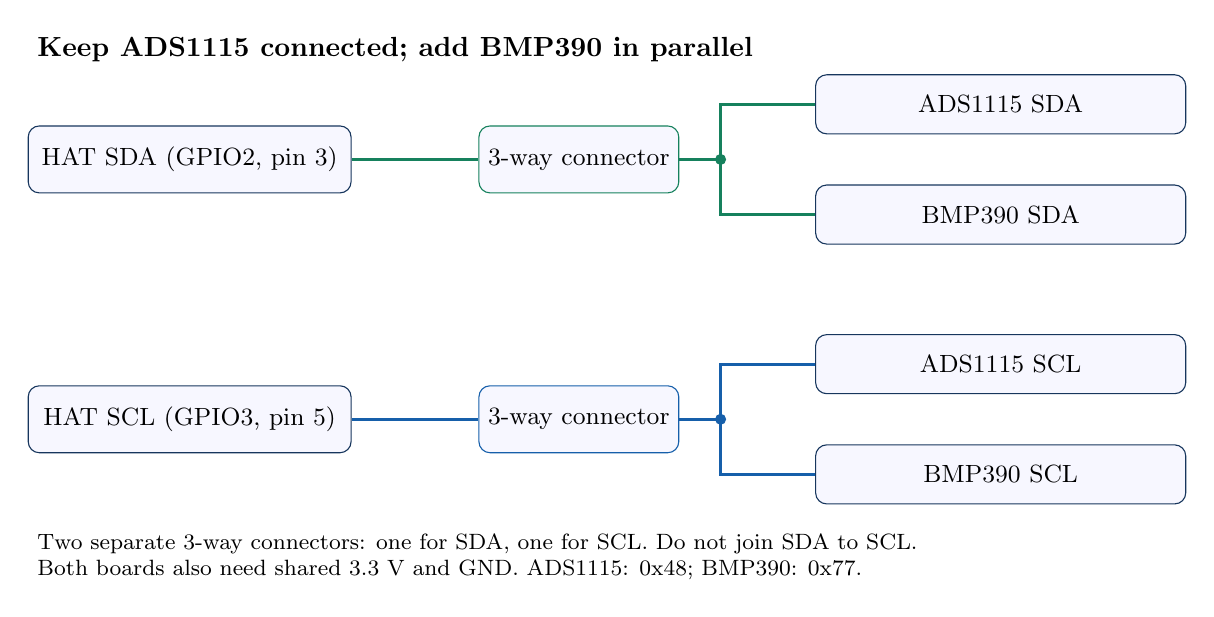
\begin{tikzpicture}[x=1cm,y=1cm]
\node[anchor=west,font=\bfseries] at (0,5.8){Keep ADS1115 connected; add BMP390 in parallel};
\foreach \y/\label/\wirecolor in {4.4/{SDA (GPIO2, pin 3)}/sda,1.1/{SCL (GPIO3, pin 5)}/scl}{
 \node[box,anchor=west,minimum width=4.1cm,minimum height=.85cm] (h) at (0,\y){HAT \label};
 \node[box,draw=\wirecolor,minimum width=2.3cm,minimum height=.85cm] (j) at (7,\y){3-way connector};
 \draw[wire,\wirecolor] (h.east)--(j.west);
 \draw[wire,\wirecolor] (j.east)--(8.8,\y)--(8.8,\y+.7)--(10,\y+.7);
 \draw[wire,\wirecolor] (8.8,\y)--(8.8,\y-.7)--(10,\y-.7);
 \fill[\wirecolor] (8.8,\y) circle(2pt);
}
\foreach \y/\text in {5.1/ADS1115 SDA,3.7/BMP390 SDA,1.8/ADS1115 SCL,0.4/BMP390 SCL}{
 \node[box,anchor=west,minimum width=4.7cm,minimum height=.75cm] at (10,\y){\text};
}
\node[align=left,anchor=west,font=\footnotesize] at (0,-.65){Two separate 3-way connectors: one for SDA, one for SCL. Do not join SDA to SCL.\\Both boards also need shared 3.3 V and GND. ADS1115: 0x48; BMP390: 0x77.};
\end{tikzpicture}
\end{document}
